\documentclass[a4paper,icelandic]{article}

%% Use utf-8 encoding for foreign characters
\usepackage[T1]{fontenc}
\usepackage[utf8]{inputenc}
\usepackage{babel}

%% Vector based fonts instead of bitmaps
\usepackage{lmodern}

%% Useful
%\usepackage{fullpage} % Smaller margins
\usepackage{enumerate}

%% Theorem
\usepackage{amsthm}
\theoremstyle{definition} \newtheorem{skilgr}{Skilgreining}
\theoremstyle{plain}      \newtheorem{setn}{Setning}
\theoremstyle{remark}     \newtheorem*{lausn}{Lausn}

%% More math
\usepackage{amsmath}
\usepackage{amssymb}

%% Code
\usepackage{verbatim}

%% Graphics
\usepackage{graphicx}
\DeclareGraphicsExtensions{.pdf}

%% Document Header
\title{\textbf{Gagnasafnsfræði}\\Verkefni 1}
\author{Hörður Freyr Yngvason}
\date{}

\begin{document}
\maketitle

Í þessu verkefni setjum við fram hönnun á gagnasafni fyrir einfaldan uppboðsvef.
Hönnunin er fyrst sett fram í einindavenslalíkani en síðan útfærð í PostgreSQL.
Til einföldunar gerum við ráð fyrir að aðeins sé notaður einn gjaldmiðill og að
öll viðskipti fari fram í heilum einingum gjaldmiðilsins.

\section{Einindavenslalíkan fyrir gagnasafnið}

\subsection{Einindin og eigindi þeirra}

Eftirfarandi eru einindin í gagnasafninu og inndregnu atriðin undir hverju
einindi eru eigindi þess. Lítum svo á að eigindi sé nauðsynlegt og ekki lykill
nema annað sé tekið fram.

\begin{description}
    \item[user] Allir notendur vefsins eru í þessari töflu.
        \begin{description}
            \item[id] Strengur, auðkenni notanda; eini lykill einindanna
                \emph{user}.
            \item[email] Strengur, netfang notanda.
            \item[name] Strengur, raunverulegt nafn notanda.
            \item[pw hash] Strengur, stytting á \emph{password hash} og er
                eigindi sem leyfir okkur að athuga hvort notandi hafi slegið inn
                rétt lykilorð. Til öryggis geymum við ekki lykilorð
                notenda í gagnagrunni, því margir nota sama lykilorðið
                oftar en einu sinni.
            \item[since] Dagsetning, hvenær tiltekinn notandi var búinn til á
                síðunni.
        \end{description}
        Nú gætum við krafist fleiri atriða, t.d. heimilisfangs o.fl. en við
        sleppum því hér, þar sem það er óþarfi; ofangreindar upplýsingar ættu að
        nægja til að hafa umsjón með notendum og þar sem öll viðskipti fara í
        gegn um greiðsluþjónustur krefjumst við þess einfaldlega fyrir viðskipti
        að notandi hafi aðgang að einhverri þeirra.
    \item[seller] Þeir notendur sem eru líka seljendur. Seljendur eru algjörlega
        háðir notendum (þ.e. veikt einindi), sjá venslin \emph{is} að neðan.
        \begin{description}
            \item[info] Strengur, pláss fyrir örstutta lýsingu frá seljanda á
                sjálfum sér.
        \end{description}
    \item[payment method] Leyfðar greiðsluþjónustur. Hugmyndin er að þær séu
        allar rafrænar og samhæfðar þannig að vefurinn geti fært frá notanda
        hvaða þjónustu sem er yfir á notanda hvaða þjónustu sem er. T.d.  PayPal
        aðgangur og greiðslukort frá Visa. Sjá nánar venslin \emph{pays using}
        og \emph{gets paid using} að neðan.
        \begin{description}
            \item[id] Strengur, auðkenni þjónustunnar; lykill sem ákvarðar hana
                ótvírætt.
        \end{description}
    \item[auction] Veikt einindi. Heldur utan um öll uppboðin í kerfinu.
        \begin{description}
            \item[id] Heiltala, lykill sem ákvarðar uppboð ótvírætt.
            \item[start, end] Dagsetningar fyrir upphaf og lok uppboðs.
            \item[min price] Heiltala, lágmarksverð sem greiða þarf fyrir
                hlutinn.
            \item[starting bid] Heiltala, verðið sem uppboðið byrjar í. Athugum
                að að engar sérstakar skorður eru settar á lágmarksverð og
                upphafsboð; með því að leyfa neikvæð gildi væri t.d. hægt að
                opna fyrir \emph{útboð}. 
        \end{description}
    \item[item] Hlutir til sölu. Þeir eru algjörlega háðir uppboðum (þ.e. veikt
        einindi) og í hverju uppboði getur aðeins einn hlutur verið til sölu.
        Athugum þó að pakki hluta er aðeins einn hlutur (sem inniheldur e.t.v.
        marga hluti).
        \begin{description}
            \item[state] Heiltala úr $0,1,2,3$ sem stendur fyrir ástand hlutar.
                Talan 0 þýðir \emph{ónýtur}, 1 þýðir \emph{virkar}, 2 þýðir
                \emph{í frábæru ástandi} og 3 þýðir \emph{nýr} (óopnaður).
            \item[label] Stuttur strengur sem mun birtast í ýmis konar listum
                yfir uppboð á síðunni.
            \item[description] Lengri lýsing á hlutnum sem birtist m.a. á
                uppboðssíðu hlutarins.
            \item[location] Strengur sem lýsir því hvar hluturinn er staðsettur. 
            \item[shipping] Heiltala með gildi 0, 1 eða 2 sem segir um afstöðu
                til póstburðar hlutar. Gildið 0 stendur fyrir \emph{engan
                flutning}, þ.e. kaupandi þarf að sækja; 1 stendur fyrir
                \emph{flutning gegn greiðslu} og 2 stendur fyrir
                \emph{flutning innifalinn}.
        \end{description}
    \item[category] Flokkar sem uppboð geta verið í.
        \begin{description}
            \item[id] Strengur, bæði lykill og nafn flokks í senn.
        \end{description}
    \item[buyer/seller review] Umsagnir kaupanda og seljanda hvor á öðrum fyrir
        tiltekin viðskipti milli þeirra. Sjá nánar venslin \emph{of1/of2} og
        \emph{deal} að neðan. Einkunnir eru heiltölur $0\dots 10$ og umsagnirnar
        eru langir strengir. Öll eigindin eru óþörf, þ.e. þau mega öll vera tóm.
        \begin{description}
            \item[rating] Einkunnin sem annar aðilinn gaf hinum fyrir
                viðskiptin.
            \item[review] Umsögnin sem annar aðilinn gaf hinum fyrir
                viðskiptin.
            \item[date] Dagsetning umsagnar.
        \end{description}
\end{description}

\subsection{Einindavensl í gagnasafninu}

Eftirfarandi eru venslin í gagnasafninu og eiginleikar þeirra. Í feitletruðu
fyrirsögnunum stendur skáletrun fyrir einindi en uppréttu orðin tákna vensl
milli þeirra.

\begin{description}
    \item[\emph{user} is \emph{seller}] 1-to-1 vensl milli notanda og seljanda
        þátttaka seljanda er algjör en ekki allir notendur þurfa að vera
        seljendur. Þessi vensl ákvarða veika einindið \emph{seller} út frá
        \emph{user}.
    \item[\emph{user} pays using \emph{payment method}] 1-to-many vensl frá
        notanda til greiðsluþjónustu. Engar aðrar þátttökuskorður. 
        Hugmyndin er að geyma þann máta sem var seinast notaður, nema notandi
        velji annað.
        \begin{description}
            \item[details] Strengur sem inniheldur einhverjar frekari
                upplýsingar um hvernig notandinn notar greiðsluþjónustuna. Til
                dæmis, ef þjónustan er PayPal, þá gæti details innihaldið
                PayPal notandanafn.
        \end{description}
    \item[\emph{seller} gets paid using \emph{payment method}] 1-to-many vensl
        frá seljanda til greiðsluþjónustu sem segja hvernig seljandi fær 
        greitt. Við setjum engar frekari þátttökuskorður því seljandi þarf ekki
        að fá greitt nema hann selji hlut. Ennfremur þarf kaupandi ekki að hafa
        áhyggjur af þessu gildi, því forsendan er að allir greiðslumátarnir séu
        samhæfðir.
        \begin{description}
            \item[details] Eins og að ofan í greiðslumáta fyrir \emph{user}.
        \end{description}
    \item[\emph{seller} has \emph{auction}] many-to-1 vensl frá seljanda til
        uppboðs sem ákvarða veika einindið \emph{auction}. Þátttaka uppboðs er
        alger en seljandi þarf ekki endilega að hafa haldið uppboð.
    \item[\emph{user} bid \emph{auction}] many-to-many vensl milli notanda og
        uppboðs án frekari þátttökuskorða. Venslin \emph{bid} standa fyrir eitt
        tilboð notanda í uppboð, e.t.v. með sjálvirkri hækkun upp að vissu
        hámarki. Notandi ber sjálfur ábyrgð á að keppa ekki óvart við sjálfan
        sig.
        \begin{description}
            \item[id] Heiltala sem við notum til að fletta upp tilboðum.
            \item[original date] Dagsetningin sem tilboðið var upphaflega lagt
                fram. Alltaf fasti.
            \item[date] Dagsetningin sem tilboðið var síðast hækkað sem tilraun
                til að slá út yfirboð, eða upphaflega dagsetningin ef það hefur
                aldrei verið hækkað.
            \item[val] Gildi tilboðsins eftir seinustu hækkun.
            \item[min] Lægsta gildi tilboðsins, þ.e. gildi þess í upphafi.
            \item[max] Hæsta gildi sem leyfilegt er að hækka boðið í sjálfvirkt. 
            \item[inc] Jákvæð heiltala sem stendur fyrir skrefstærð sjálfvirkrar
                hækkunar. Reynum ávallt að hækka boðið eins lítið og hægt er um
                margfeldi af skrefstærð, nema eini kosturinn sé hæsta leyfða
                gildið.
        \end{description}
        Af þessu sést að öll tilboð eru í raun sjálvirk, en ef \emph{min} og
        \emph{max} eru sama gildið þá er aldrei nein hækkun framkvæmd. Við
        komumst upp með að haga þessu svona, þ.e. að nota uppfærslur í stað þess
        að bæta sjálfvirkt við nýju tilboði fyrir hækkanir, því ekki þarf að
        sýna sögu tilboða í uppboð á síðunni. Aðeins þarf að vera unnt að
        úrskurða hæsta tilboð í uppboð að hverju sinni og þau tilboð notanda sem
        eru opin (þ.e. tilboð í ólokið uppboð).
    \item[\emph{user} deal \emph{auction}] Many-to-1 vensl milli notanda og
        uppboðs án frekar þátttökuskorða. Þessi vensl standa fyrir innsiglun
        kaupsamnings eftir lok uppboðs. Upphaflega var ætlunin að láta samning
        vera tengdan beint við tilboð á einhvern hátt og ákvarða þannig uppboð
        og notanda, en því fylgdu erfiðleikar í að takmarka fjölda samninga
        fyrir hvert tilboð.
        \begin{description}
            \item[id] Heiltala sem við notum sem auðkenni samnings.
            \item[val] Umsamin upphæð á kaupum; ætti venjulega að vera upphæð
                tilboðsins sem vann uppboðið.
            \item[date] Dagsetningin sem samningurinn var framvæmdur (felur
                a.m.k. í sér greiðsluskuldbindingu).
        \end{description}
    \item[\emph{buyer/seller review} of (\emph{user} deal \emph{auction})]
        1-to-1 vensl milli umsagna og kaupsamnings, full þátttaka umsagna í
        venslunum en samningur þarf ekki að hafa neina umsögn. Venslin ákvarða
        veika einindið \emph{buyer/seller review}. Hugmyndin er að leyfa aðeins
        umsögn milli notenda fyrir stunduð viðskipti, en til að gefa kvika mynd
        af seljendum og kaupendum verður að leyfa umsögn fyrir sérhver
        viðskipti; annars gætu stórnotendur, sem hafa hegðað sér vel framan af,
        skyndilega breytt hegðun sinni til hins verra án verulegra breytinga í
        umsögnum.
    \item[\emph{auction} is in \emph{category}] Many-to-many vensl milli uppboða
        og flokka án frekari þátttökuskorða.
    \item[\emph{auction} selling \emph{item}] 1-to-1 vensl milli uppboða og
        hluta með fullri þáttöku beggja aðila, auk þess að hlutur á ekki að vera
        til í gagnagrunninum nema hann sé á uppboði. Þ.e. uppboð ákvarðar veika
        eigindið \emph{item} um þessi vensl.
\end{description}

\subsection{Teikning einindavenslaritsins}

Einindavenslaritið var teiknað í forritinu Dia, sjá mynd \ref{fig:erd} á bls.
\pageref{fig:erd}.

\begin{figure}[h]
    \begin{center}
        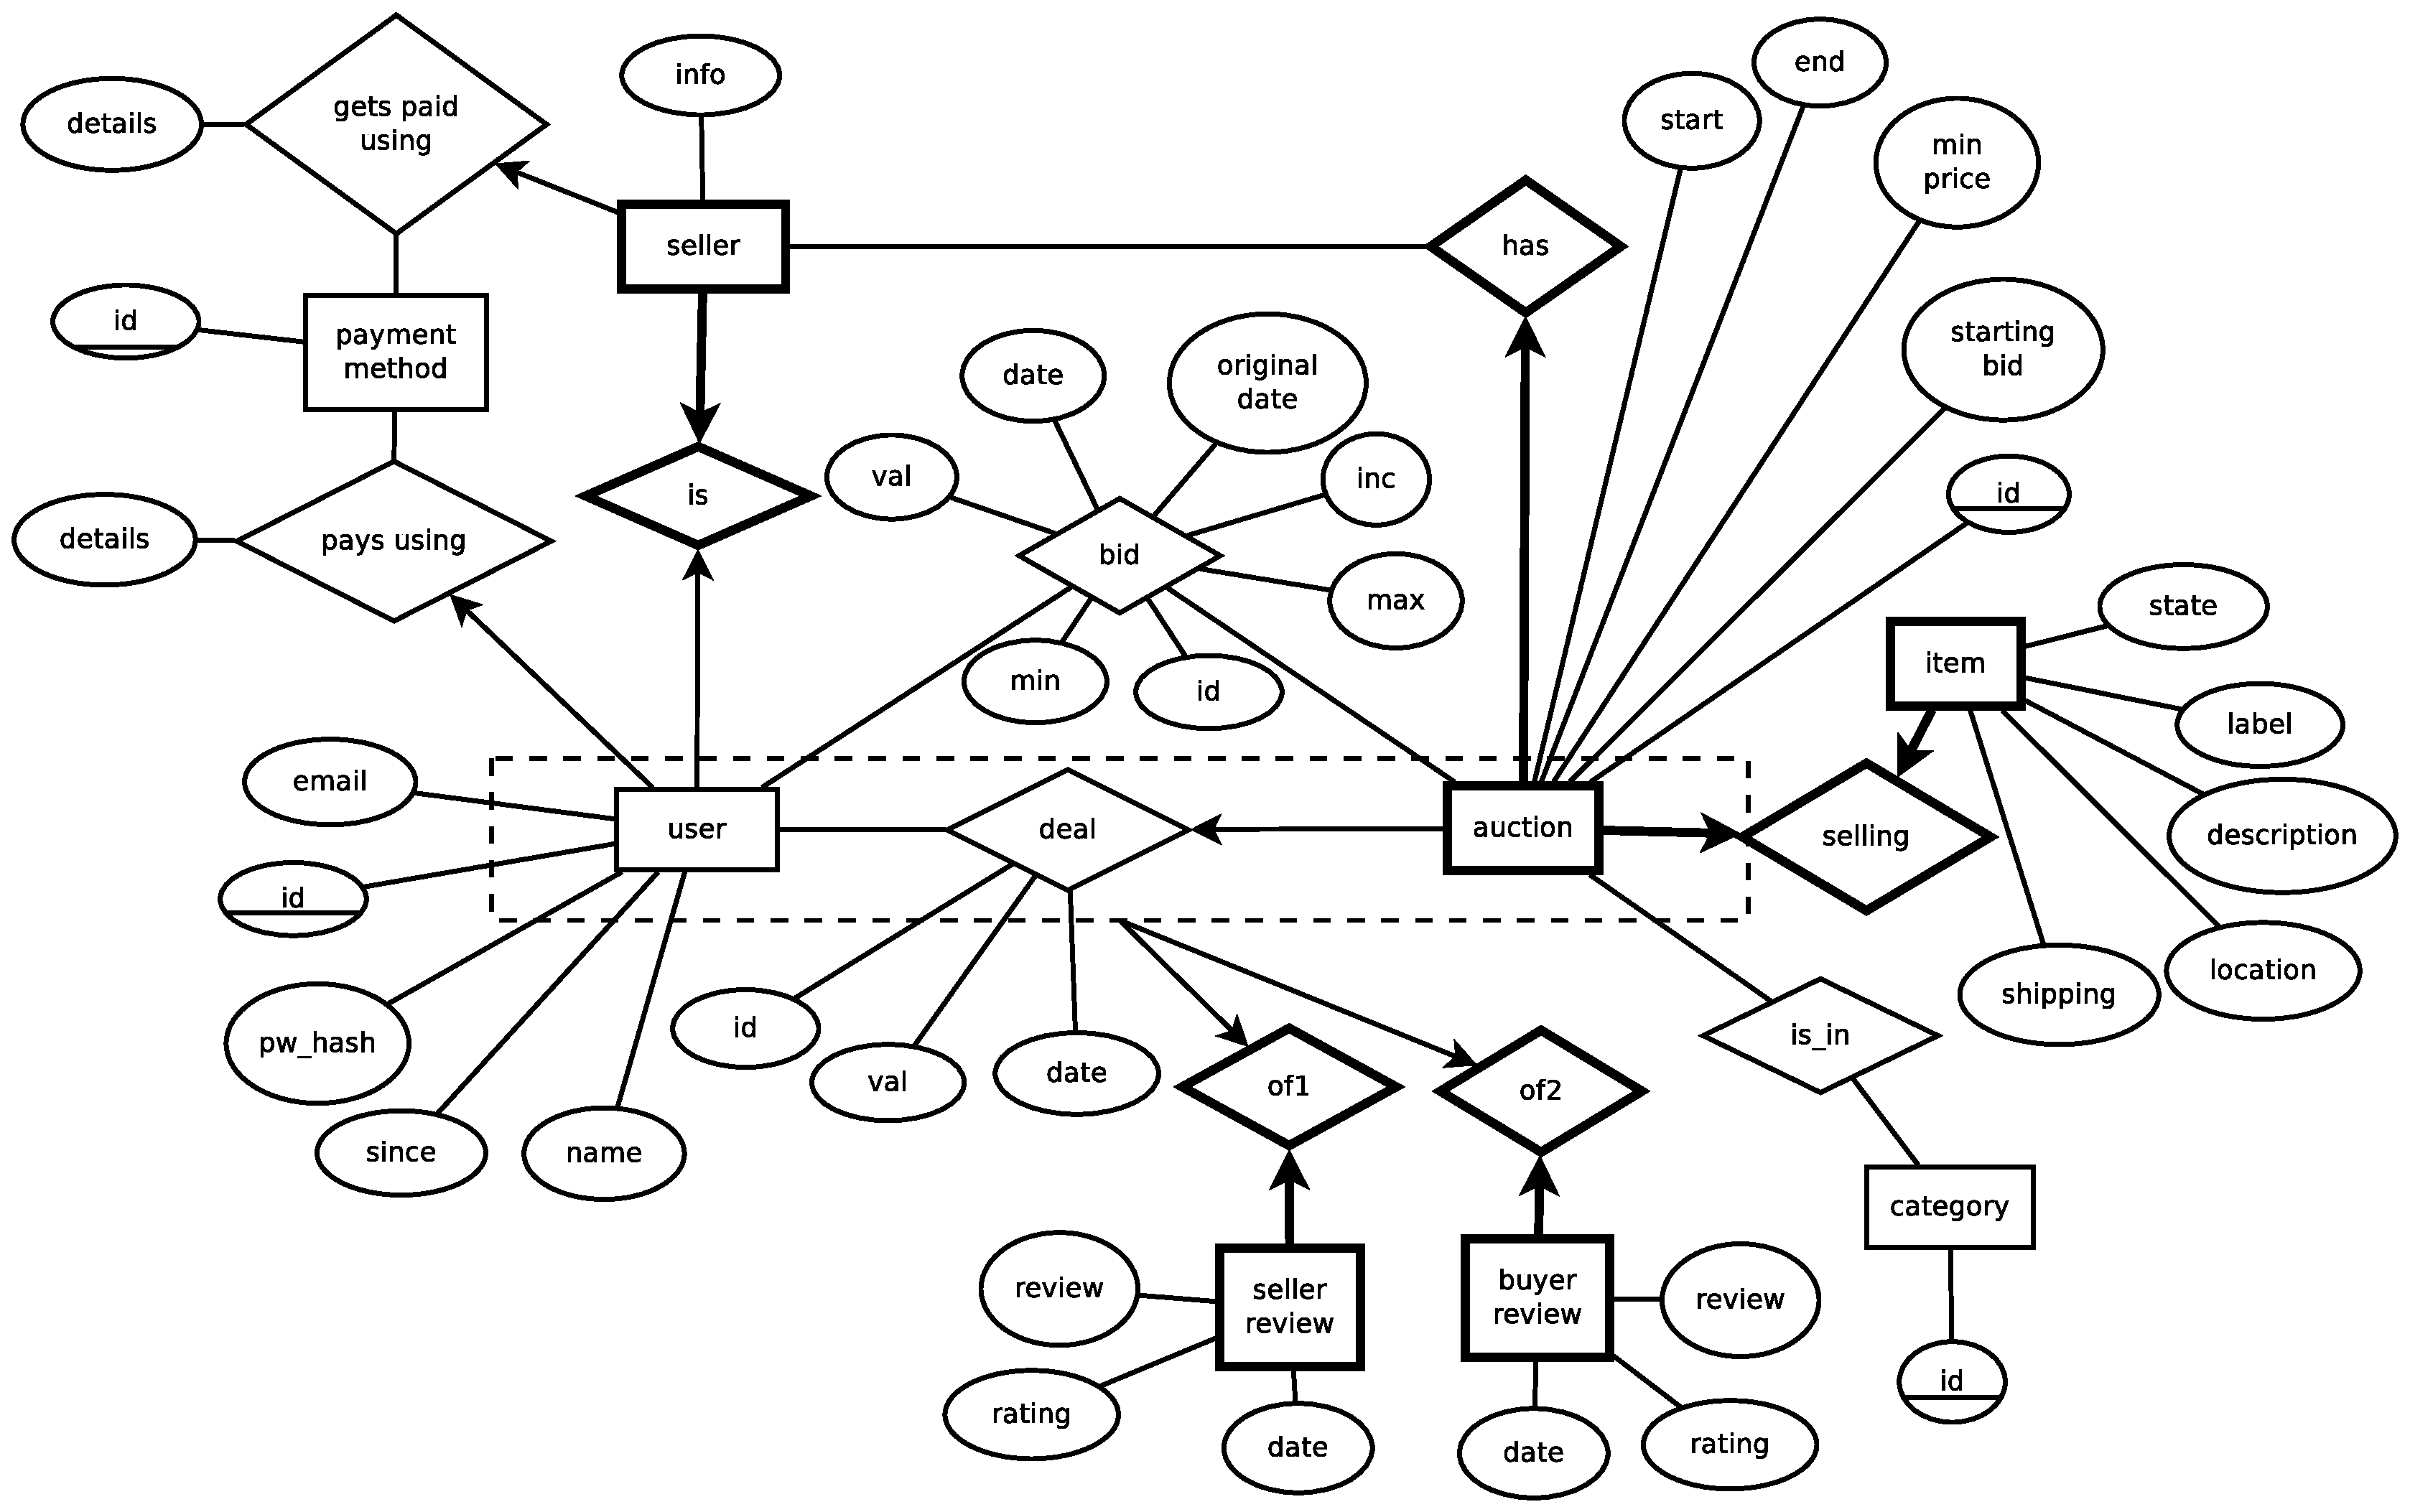
\includegraphics[width=0.96\textheight,angle=-90]{schema.eps}
    \end{center}
    \caption{Einindavenslaritið eins og því er lýst í grein 1}
    \label{fig:erd}
\end{figure}

\section{PostgreSQL töflur gagnasafnsins}

Í gagnasafninu eru eftirfarandi töflur

\begin{description}
    \item[\texttt{t\_user}] Tafla allra notenda á vefnum. Inniheldur 
        \begin{itemize}
            \item allt úr \emph{user} einindinu
            \item venslin \emph{pays using} ef þau eru til staðar
            \item allt úr \emph{seller} ef notandi er seljandi og tilsvarandi
                vensl \emph{gets paid using} ef þau eru til staðar.
        \end{itemize}
    \item[\texttt{t\_auction}] Tafla allra uppboða á vefnum. Inniheldur
        \begin{itemize}
            \item allt úr \emph{auction} einindinu og tilsvarandi hlut
                \emph{item} (með öllum eigindum)
            \item venslin \emph{has} við \emph{seller}.
        \end{itemize}
    \item[\texttt{t\_bid}] Inniheldur venslin \emph{bid} og ekkert annað.
    \item[\texttt{t\_deal}] Inniheldur samningsvenslin \emph{deal} og
        tilsvarandi umsagnir úr \emph{review}.
    \item[\texttt{t\_category}] Allir flokkar og ekkert annað.
    \item[\texttt{t\_auction\_category}] Inniheldur venslin \emph{is in} milli
        flokka og uppboða og ekkert annað.
    \item[\texttt{t\_payment\_method}] Inniheldur greiðsluþjónusturnar og ekkert
        annað.
\end{description}
Ef ekkert hefur mistekist ætti venslalíkanið með þessum samsvörunum við
töflurnar að vera strangt hlutmengi í SQL-skilgreiningunum. Þ.e. ætlunin er að
allar skorður í venslalíkaninu komi fram í SQL-skilgreiningunum, en greinilega
eru sumar skorður, t.d. \verb|auction_start < auction_end|, sem ekki er hægt að
tjá á myndinni.

Eftirfarandi eru síðan töfluskilgreiningarnar sjálfar
\verbatiminput{auction-schema.sql}

\section{Sýnisgögn fyrir gagnasafnið}

Eftirfarandi gögn voru sett inn í safnið
\verbatiminput{auction-data.sql}

\section{Valdar fyrirspurnir í gagnasafnið}

\subsection{Innskráningarsíða}

Athuga á hvort innslegið notandanafn og lykilorð finnist í gagnasafninu. Útfærum
þetta sem hjálparfall \verb|authenticate_user| sem tekur notendanafn og hash af
lykilorði og skilar bool gildi, sem er satt þ.þ.a.a. til sé notandi með þetta
hash af lykilorði.
\verbatiminput{gsf.4a.sql}

\subsection{Upphafssíða notanda}

Sýna á \emph{opin tilboð} notanda, alla flokka, nýjustu 5 uppboðin og e.t.v.
eitthvað fleira. Lítum svo á að tilboð frá notanda sé opið e.f.f. tilsvarandi
uppboð þess er enn í gangi. Útfærum:
\verbatiminput{gsf.4b.sql}

\subsection{Uppboðssíða hlutar}
Á uppboðssíðu hlutar eiga að vera upplýsingar um hlutinn og stöðu uppboðsins.
Þar er sýnt núverandi hæsta tilboð, hversu mikill tími er eftir af uppboðinu og
upplýsingar um seljandann (meðaleinkunn og fjöldi sala). Útfærum:
\verbatiminput{gsf.4c.sql}

\subsection{Tilboð gert í hlut}

Sýna á fyrirspurn til að gera tilboð í hlut ásamt kveikju ef notandinn vill
sjálvirkt boð. Við höfum þegar afgreitt kveikjuhlutann með því að láta öll boð
vera sjálfvirk og láta síðan kveikjufallið \verb|autobid_raise| úrskurða nýtt
besta boð fyrir hverja nýja innsetningu í \verb|t_bid|. Okkur nægir því
eftirfarandi innsetningarfall:
\verbatiminput{gsf.4d.sql}

\subsection{Skráning einkunna og umsagna}

Rifjum upp að umsagnir og einkunnir eru háðar því að viðskipti hafi verið
stunduð. Þ.e. kaupandi getur gefið seljanda einkunn og umsögn fyrir hvern gerðan
samning, og öfugt. Við útfærum því:
\verbatiminput{gsf.4e.sql}

\subsection{Upplýsingasíða um seljanda}
Koma þarf fram hve lengi seljandi hefur verið skráður, meðaleinkunn og síðustu 5
umsagnir um hann. Fyrir fyrstu 2 atriðin notum við beint sýnina
\verb|seller_stats| úr 4.3 og einskorðum hana við tiltekinn notanda.
\verbatiminput{gsf.4f.sql}

\subsection{Nýr notandi}
Setjum inn nýjan notanda með fallinu
\verbatiminput{gsf.4g.sql}

\subsection{Nýr seljandi}
Setjum inn nýjan seljanda í tveimur skrefum. Búum fyrst til nýjan notanda eins
og að ofan, ef hann er ekki til. Uppfærum síðan þann notanda með tilheyrandi
upplýsingum:
\verbatiminput{gsf.4h.sql}

\end{document}
